Under the understanding that the reactions of interest for this work follow a pseudo-first-order model, a theoretical framework is needed to compare our findings. To figure out the characteristic rate constant $k$ of a reaction, we want to model the interaction between the reactants, whether it be neutral-neutral, to ion-dipole. To do this, we consider adiabatic capture theory, a study of the long range potentials between particles. A caveat is that the adiabatic capture theory is long ranged, only finding the rate at which a collision will occur, not necessarily when a reaction will happen. The probability of a reaction occurring requires modeling of short range interactions within the reaction complex, but understanding capture theory will yield the maximally allowed rate of reactions, if all collisions lead to a reaction.

\subsection{Generalized Rate Constant Derivation} \label{sec: ACT}
A general method of calculating the rate constant of two particles with a given potential, finding the collisional cross section, which is then averaged over a velocity distribution to find the rate constant.\cite{Zhang2017} The interaction potential of two reactants is generally defined as
\begin{equation}
    V(r) = \sum_n - \frac{C_n}{r^n}
\end{equation}
where $C_n$ is the interaction coefficient of order $n$. We may write the effective potential in the center of mass frame as
\begin{equation}
    V_{\mathrm{eff}} = \frac{l^2}{2 \mu_R r^2} + V(r)\label{eq: veff}
\end{equation}
where $\mu_R=m_1 m_2/(m_1 + m_2)$ is the reduced mass of the two particles. The competition between the repulsive and attractive terms creates a barrier as seen in Figure \ref{fig: veff}.
\begin{figure}[H]
	\centering
	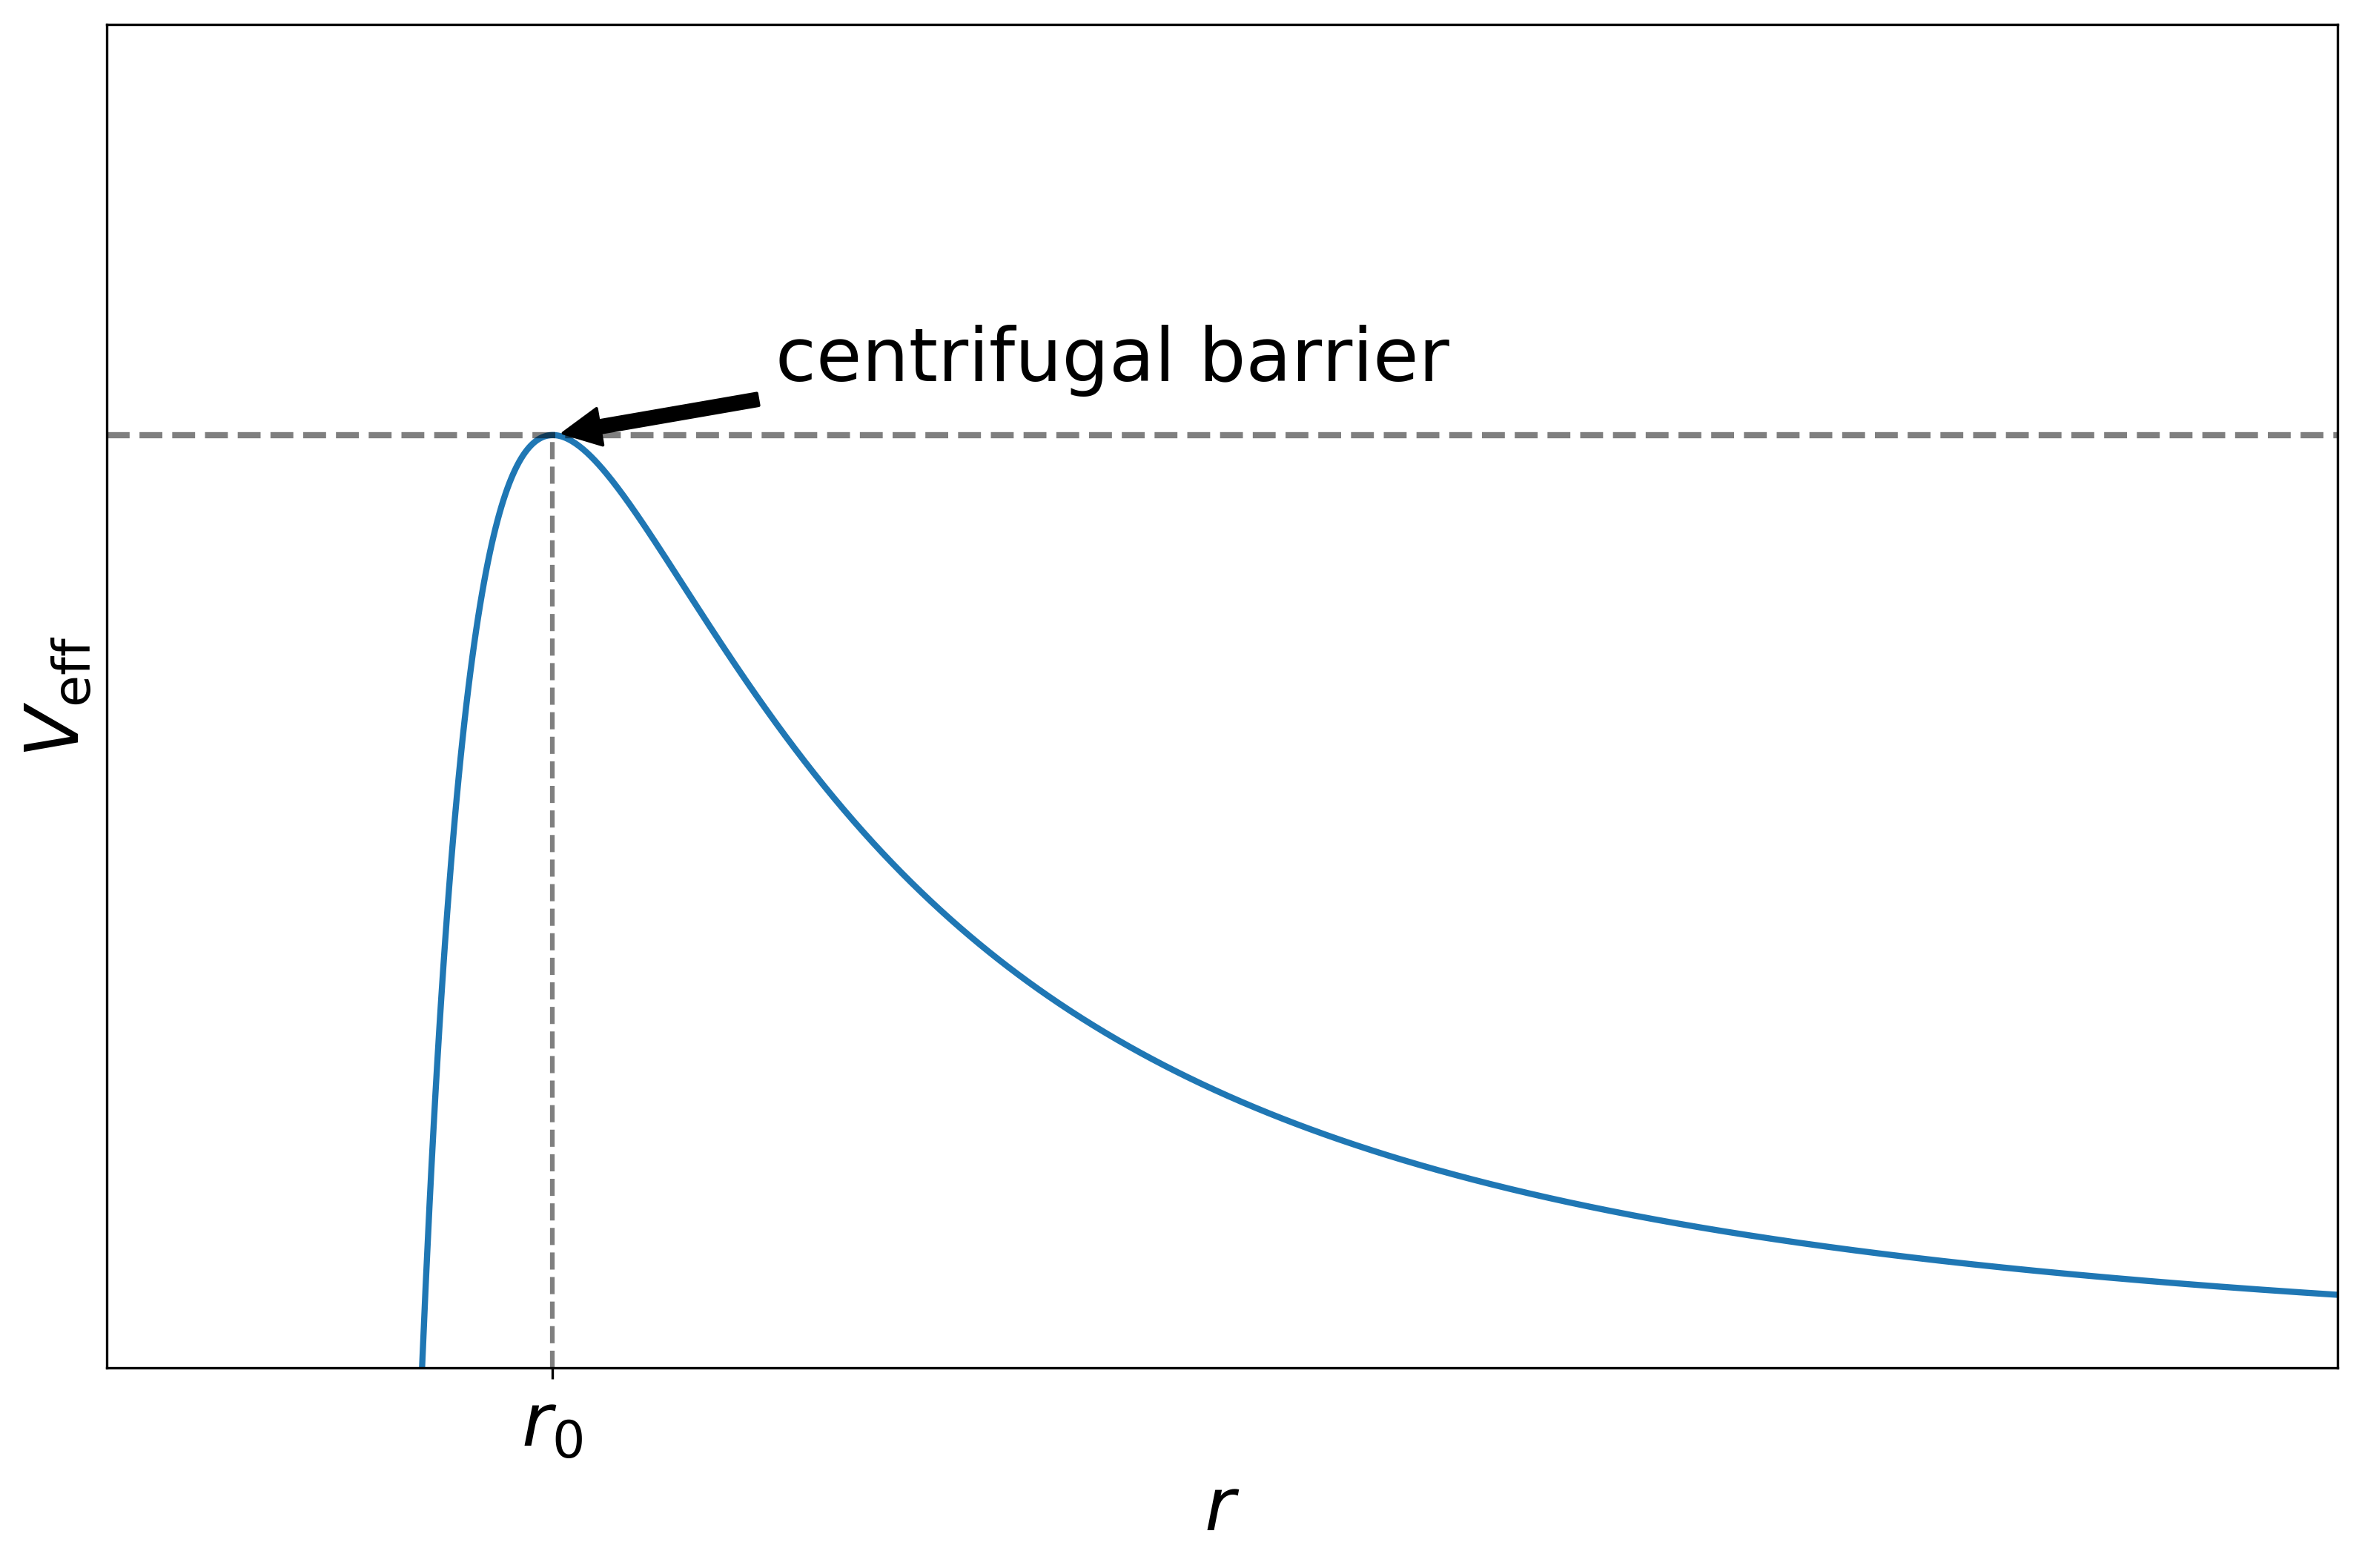
\includegraphics[width=0.8\textwidth]{images/v_eff.png}
	\caption{An arbitrary effective potential of an monopole-induced-dipole interaction. The maximum of the potential at $r_0$ creates a centrifugal barrier. Only particles with $E_{\mathrm{col}} > V_{\mathrm{eff}}$ surmount the barrier and collide.}
	\label{fig: veff}
\end{figure}
To find the condition for a collision to occur, we first find the position $r_0$ corresponding to the maximum of the effective potential, which is the value of the centrifugal barrier.
\begin{align*}
    \frac{\partial V_{\mathrm{eff}}}{\partial r}\bigg|_{r_0} & = 0 \\
    \therefore r_0 & = \left(\frac{n \mu_R C_n}{l^2}\right)^{1/n-2}
\end{align*}
Substituting $r_0$ back into equation $\ref{eq: veff}$, we find the maximal value of the effective potential:
\begin{equation}
    V_{\mathrm{eff}}(r_0) = \left(\frac{l^2}{\mu_R}\right)^{\frac{n}{n-2}} \frac{n-2}{2n}(n C_n)^{-\frac{2}{n-2}}
\end{equation}
This then defines the energy necessary for a collision, for if $E_{\mathrm{col}}$ exceeds $V_{\mathrm{eff}}(r_0)$, the reactants will be able to surmount the centrifugal barrier and collide. For the condition where $V_{\mathrm{eff}}(r_0) = E_{\mathrm{col}} = \frac{1}{2}\mu_R v^2$, we define the maximum value for the angular momentum $l$ and the impact parameter $b$.
\begin{align*}
    l_{\max} & = (\mu_R n)^{1/2}(C_n)^{1/n} \left(\frac{2 E_{col}}{n-2}\right)^{\frac{n-2}{2n}} \\
    b_{\max} & = \frac{l_{\max}}{\mu_R v}
\end{align*}
We can then define a collision cross section dependent on the collision energy:
\begin{align*}
    \sigma(E_{col}) & = \pi b^2_{\max} \\
    & = \frac{\pi}{2} n \left(\frac{2}{n-2}\right)^{\frac{n-2}{2}} \left(\frac{C_n}{E_{col}}\right)^{\frac{2}{n}}
\end{align*}
Integrating the collision cross section with a Maxwell Boltzmann distribution yields a generalized rate constant as a function of temperature and $n$.
\begin{align}
    k(T) & = \int_0^{\infty} v f(v) \sigma(v) dv \label{eq: k int} \\
    & = \sqrt{\frac{2 \pi}{\mu_R}}n\left(\frac{2}{n-2}\right)^{\frac{n-2}{2}}C_n^{2/n}(k_B T)^{\frac{n-4}{2n}}\Gamma\left(2-\frac{2}{n}\right) \label{eq: k(T)}
\end{align}
For instance, the monopole-induced-dipole potential of order $n=4$ has the form and rate constant
\begin{align}
	V_L & = -\frac{\alpha q^2}{2r^4} \label{eq: V_L} \\
	k(T) & = 2\pi q \sqrt{\frac{\alpha}{\mu_R}} \label{eq: k langevin}
\end{align}
where $\alpha$ is the polarizability of the neutral reactant, and $q$ is the monopole charge. The corresponding $k(T)$ in equation \ref{eq: k langevin} is known as the Langevin rate constant, which is famously temperature independent.

\subsection{Average Dipole Orientation (ADO)}

Unlike the general derivation for adiabatic capture theory outlined in the previous section. We now want to calculate the rate constant for an interaction with more than just an $r$ dependence. The monopole-dipole interaction term is not radially symmetric because the dipole may be oriented at an angle $\theta$ with respect to the inter-nuclear axis as shown in Figure \ref{fig: dipole angle}. The potential can be written as
\begin{equation}
	V_D(r, \theta) = -\frac{q\mu_D}{r^2} \cos(\theta).
	\label{eq: V_D}
\end{equation}

\begin{figure}[H]
	\centering
	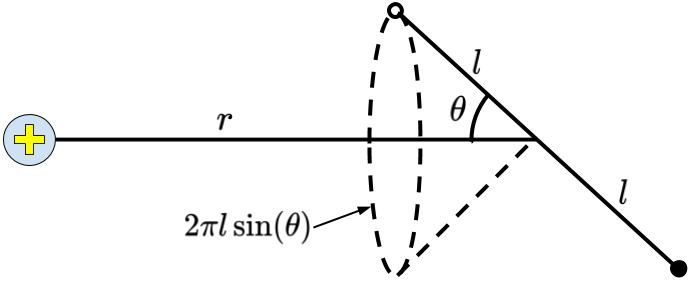
\includegraphics[width=0.6\textwidth]{images/dipole_angle.png}
	\caption{A monopole and a dipole of length $2l$ separated by distance $r$ where the dipole is oriented with angle $\theta$ with respect to the internuclear axis. The circumference that the dipole traces at a given angle $\theta$ is shown by the dotted circle.}
	\label{fig: dipole angle}
\end{figure}

The method outlined in section \ref{sec: ACT} finds the rate constant by dealing with a two body problem only needing to consider the $r$ degree of freedom. The inclusion of the angle $\theta$ in the potential in equation \ref{eq: V_D} complicates this. We could assume that the dipole "locks" onto the monopole and always has an angle $\theta=0$, but that has been shown to not agree with experimental results.\cite{Su1973a} Instead, it is more appropriate to determine an averaged $\theta$ as a function of $r$. The derivation for the average dipole orientation theory (ADO) pioneered and expanded on by Su and Bowers is used.\cite{Su1973, Su1973a} Considering a monopole and dipole, the interaction potential will include both potential terms \ref{eq: V_L} and \ref{eq: V_D}
\begin{equation}
    V(r) = -\frac{\alpha q^2}{2r^4} - \frac{q\mu_D}{r^2} \cos\left(\bar{\theta}(r)\right)
    \label{eq: V_L+V_D}
\end{equation}
where $\bar{\theta}(r)$ is the averaged orientation of the dipole angle as a function of internuclear distance $r$. This is given by a weighted average
\begin{equation}
	\bar{\theta} = \dfrac{\int \theta P(\theta) d\theta}{\int P(\theta) d\theta} \label{eq: avg theta}
\end{equation}
where $P(\theta)$ is the probability of finding the dipole oriented with angle $\theta$. It may seem daunting to find the form of $P(\theta)$, but since it is in both numerator and denominator of equation \ref{eq: avg theta}, only the dependence on $\theta$ is needed. In particular, two proportionalities with respect to $\theta$ arise.
\begin{enumerate}
	\item If the dipole is spinning with some angularly dependent angular velocity, $\dot{\theta}(\theta)$, the dipole spends less time in certain orientations. Thus, the probability of finding the dipole in a given orientation is inversely proportional to its angular velocity.
	\begin{equation}
		P(\theta) \propto 1/\dot{\theta} \label{eq: prop case 1}
	\end{equation}
	\item At any given angle $\theta$ the dipole may trace out a circle with circumference $C = 2\pi l \sin(\theta)$, seen in Figure \ref{fig: dipole angle}. This circumference out is akin to the allowed "phase space" for each angle $\theta$, thus angles with greater "phase space" are more likely to be observed.
	\begin{equation}
		P(\theta) \propto \sin(\theta) \label{eq: prop case 2}
	\end{equation}
\end{enumerate}

Combining the proportionalities of equations \ref{eq: prop case 1} and \ref{eq: prop case 2} yields
\begin{align}
    P(\theta) & \propto \frac{\sin(\theta)}{\dot{\theta}}. \label{eq: prob}
\end{align}
We can relate the angular velocity to the angular kinetic energy and the total rotational energy in the system.
\begin{align}
    KE_{rot} & = \frac{1}{2}I\dot{\theta}^2 \nonumber \\
    E_{tot} & = KE_{rot} + V_D \label{eq: Etot}
\end{align}
Redefining equation \ref{eq: prob} with equation \ref{eq: Etot}, we find the form
\begin{equation}
    P(\theta) \propto \frac{\sin(\theta)}{\sqrt{E_{rot}-V_D}}. \label{eq: p theta}
\end{equation}
Combining equations \ref{eq: p theta} and \ref{eq: avg theta} yields a fuller form of the averaged dipole angle.
\begin{equation}
    \bar{\theta} = \dfrac{\displaystyle \int\frac{\theta \sin(\theta)d\theta}{\sqrt{E_{rot}+q\mu_D/r^2 \cos(\theta)}}}{\displaystyle \int\frac{\sin(\theta)d\theta}{\sqrt{E_{rot}+q\mu_D/r^2 \cos(\theta)}}} \label{eq: avg theta int}
\end{equation}

We may be temped to simply integrate over all angles $\theta$, but there are two situations that split the solution into two separate calculations.
\begin{enumerate}
	\item $E_{rot} = E_1 < \frac{q \mu_D}{r^2}$:
	There is not enough rotational energy to overcome the dipole locking and is constrained to a maximal angle $K$. The behavior is oscillatory around the dipole-locking condition, but never fully averages to 0, as shown in Figure \ref{fig: theta1}.
	\begin{equation*}
		E_1=-\frac{q \mu_D}{r^2}\cos(K)
	\end{equation*}
	When substituted into equation \ref{eq: avg theta int}, we find:
	\begin{equation}
	    \bar{\theta}_1(r) = \dfrac{\displaystyle\int_0^K \frac{\theta \sin(\theta) d \theta}{\sqrt{\cos(\theta) - \cos(K)}}}{\displaystyle\int_0^K \frac{\sin(\theta) d \theta}{\sqrt{\cos(\theta) - \cos(K)}}} \label{eq: theta1}
	\end{equation}
	After integration by infinite series,
	\begin{align*}
	    \bar{\theta}_1 & = \frac{2 \sqrt{2}A}{\sqrt{1-\cos(K)}} \\
	    \text{where }A & \equiv \int_0^{\pi/2} \frac{a^2 \cos(\phi)^2 d\phi}{\sqrt{1-a^2 \sin(\phi)^2}} \\
	    a & \equiv \sin\left(\frac{K}{2}\right).
	\end{align*}
	\begin{figure}[H]
		\label{fig: theta1}
		\centering
		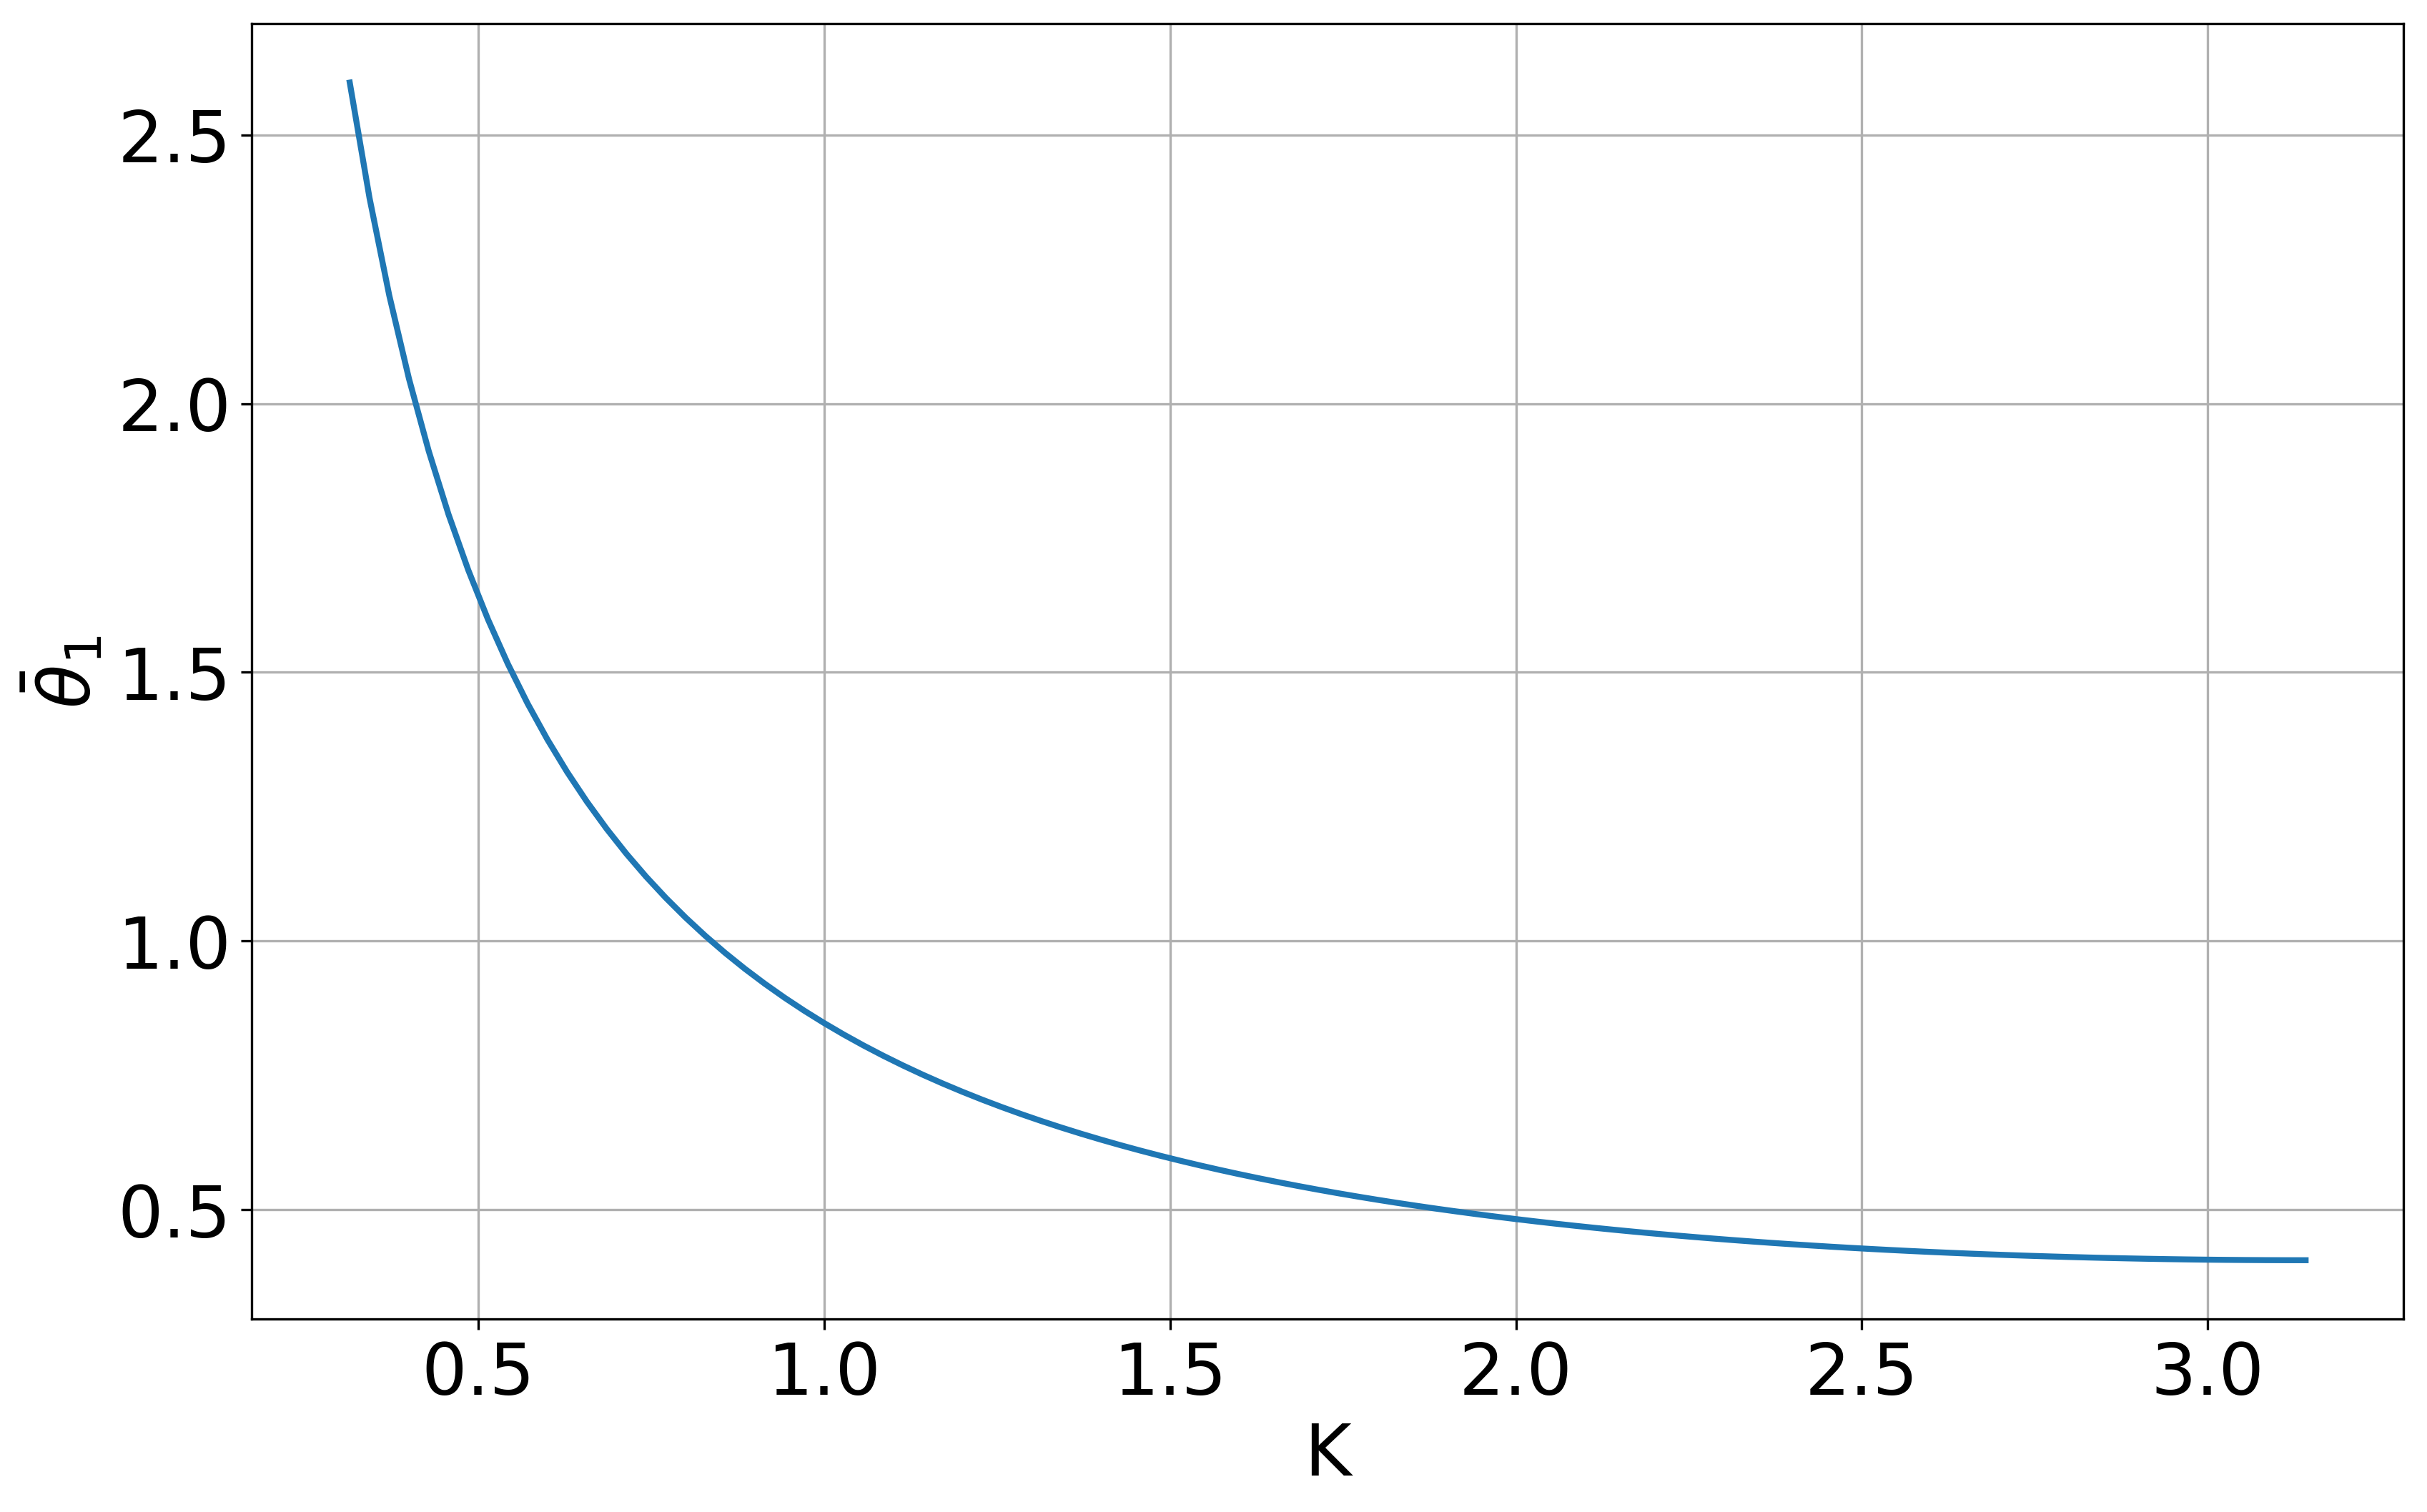
\includegraphics[width=0.8\textwidth]{images/ADO_theta1.png}
		\caption{Numerical solutions for equation \ref{eq: theta1} as a function of maximum angle $K$. As $K$ increases the value of $\bar{\theta}$ decreases but never fully reaches 0 where there would be full dipole-locking.}
	\end{figure}

	\item $E_{rot} = E_2 > \frac{q \mu_D}{r^2}$:
	The rotational energy is enough to overcome the dipole locking and $\theta$ can swing around in a complete circle. We no longer have bounds on the angles the dipole is allowed over, but the behavior is still dependent on the strength of the internal energy and monopole-dipole interaction.
	\begin{equation}
	    \bar{\theta}_2(r)  = \dfrac{\displaystyle\int_0^\pi \frac{\theta \sin(\theta) d\theta}{\sqrt{E_2 + q \mu_D/r^2 \cos(\theta)}}}{\displaystyle\int_0^\pi \frac{\sin(\theta) d \theta}{\sqrt{E_2 + q \mu_D/r^2 \cos(\theta)}}} \label{eq: theta2}
	\end{equation}
	To gain some intuition on the behavior of $\bar{\theta}_2$, we can rewrite equation \ref{eq: theta2} in the limit that $E_2 \gg \frac{q \mu_D}{r^2}$.
	\begin{equation*}
		\bar{\theta}_2 = \dfrac{\displaystyle\int_0^\pi \theta \sin(\theta) d\theta}{\displaystyle\int_0^\pi \sin(\theta) d \theta} = \dfrac{\pi}{2}
	\end{equation*}
	We see that when the rotational energy is much larger than the interaction potential, we reduce the angular proportionality $P(\theta)$ to just the second proportionality case in equation \ref{eq: prop case 2}. Since the angles are weighted by their respective "phase space", $\theta=\pi/2$ becomes the dominant orientation. This is verified in the plotted numerical solutions to equation \ref{eq: theta2} in Figure \ref{fig: theta2}
	\begin{figure}[H]
		\centering
		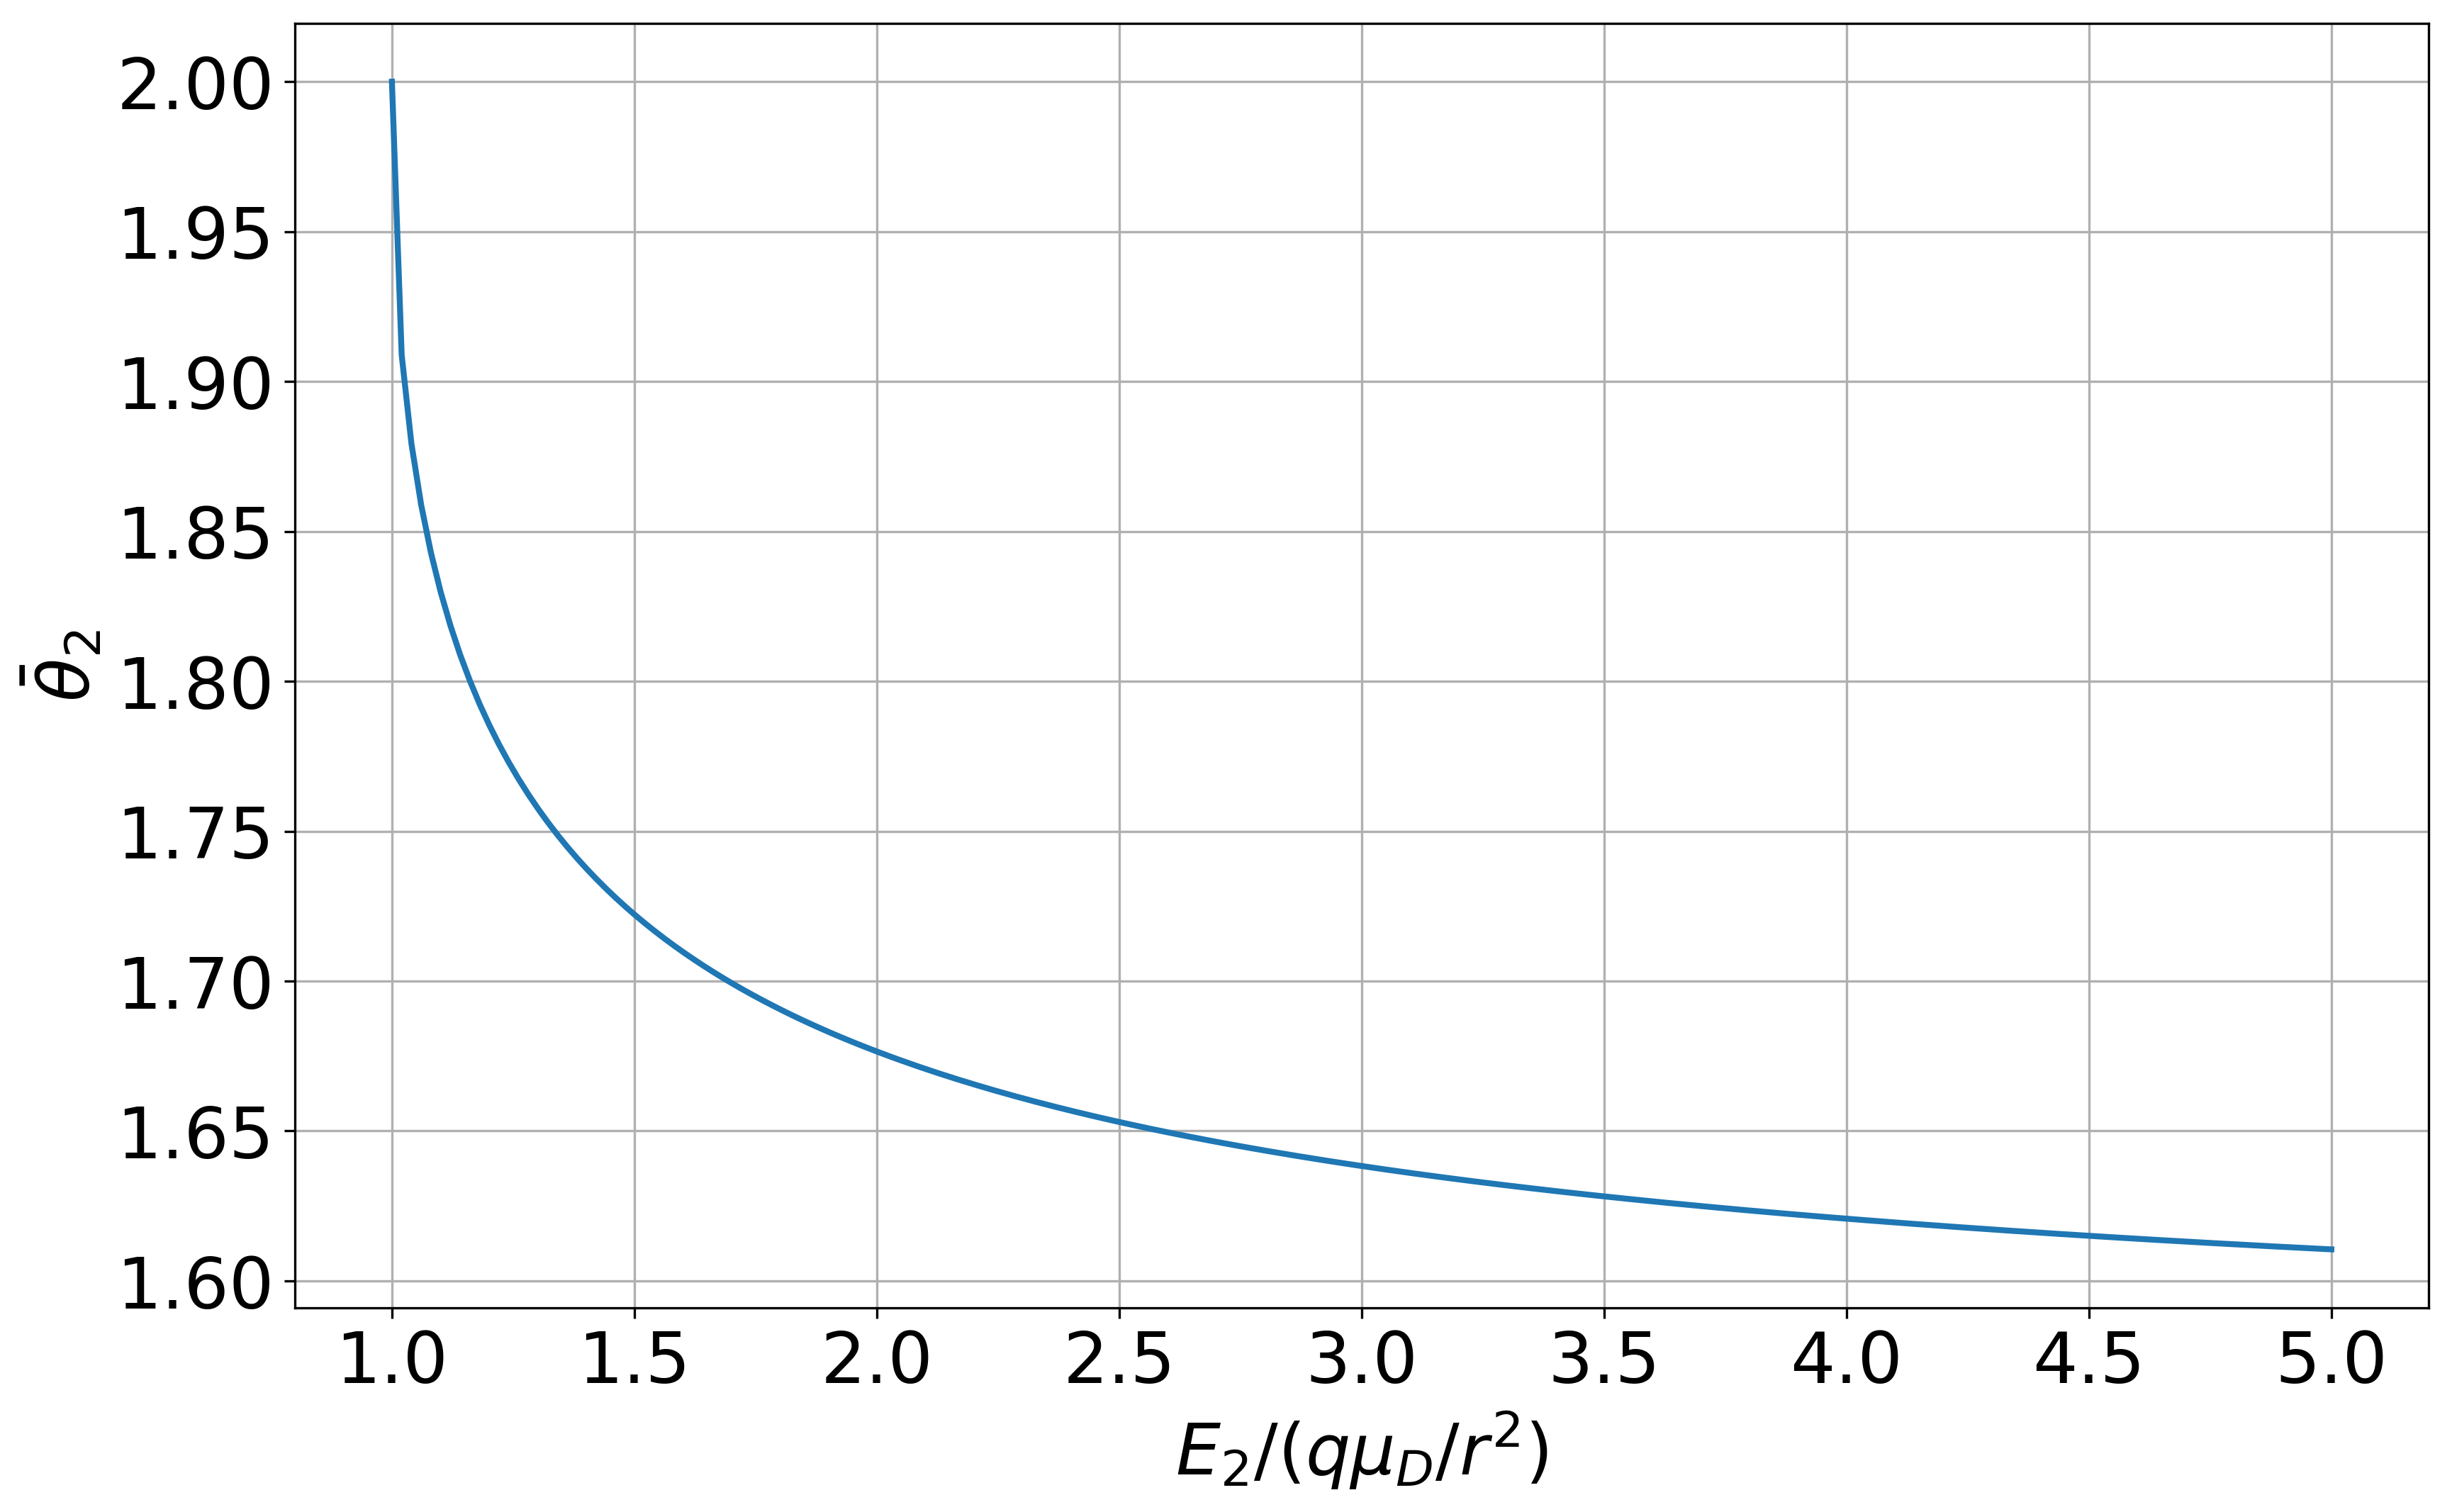
\includegraphics[width=0.8\textwidth]{images/ADO_theta2.png}
		\caption{Numerical solutions to equation \ref{eq: theta2} as a function of the ratio of rotational energy and the monopole-dipole term. As the energy ratio increases, the more $\bar{\theta}_2$ tends towards $\pi/2$.}
		\label{fig: theta2}
	\end{figure}
\end{enumerate}

Let's say we have the forms for $\bar{\theta_1}(r)$ and $\bar{\theta_2}(r)$, we want to write down the full form of $\bar{\theta}(r)$. We can combine the two weighted by the probability of each as a function of internal energy.
\begin{equation}
    \bar{\theta}(r) = \bar{\theta}_1(r) F_1(r) + \bar{\theta}_2(r) F_2(r) \label{eq: weighted theta}
\end{equation}
Where the weightings $F_i(r)$ are related to the Boltzmann distribution of internal states given by
\begin{equation*}
    P(\epsilon) d\epsilon = \frac{1}{k_BT}e^{-\frac{\epsilon}{k_BT}}d\epsilon.
\end{equation*}
For diatomics, the energies of rotational states is defined as
\begin{equation*}
    \epsilon = B_e J(J+1)
\end{equation*}
where the rotational constant is $B_e=\hbar^2/(2\mu_R r^2)$, $\mu_R$ is the reduced mass of the molecule, and $r$ is the inter-nuclear separation.

To find the rate constant, the same process described in the general adiabatic capture theory derivation can be applied to the interaction potential in equation \ref{eq: V_L+V_D}). The centrifugal barrier is
\begin{equation*}
	V_{\mathrm{eff}}(r_0) = \dfrac{l^2}{2 \mu_R r_0^2} - \dfrac{q^2 \alpha}{2r_0^4} - \dfrac{q\mu_D}{r_0^2} \cos(\bar{\theta}(r_0)).
\end{equation*}
Solving for the situation where $E_{\mathrm{col}} = V_{\mathrm{eff}}$, we find the maximum allowed angular momentum to be
\begin{equation*}
	l_{\max} = \sqrt{2\mu_D \left(E_{\mathrm{col}} + q \mu_D \cos(\bar{\theta}(r_o)) + \dfrac{q^2 \alpha}{2 r_0^2}\right)}
\end{equation*}
where the impact parameter is again defined as $b=l/(\mu_R v)$. In terms of the averaged angle, we can then find an averaged collision cross section of the form
\begin{equation*}
	\langle \sigma \rangle = \dfrac{2 \mu_R^2}{v^2} \sqrt{E_{\mathrm{col}} + q \mu_D \cos(\bar{\theta}(r_o)) + \dfrac{q^2 \alpha}{2 r_0^2}}.
\end{equation*}
We now have all the components necessary to find the rate constant by integrating over a translational velocity distribution
\begin{equation*}
	k(T) \int_0^\infty v f(v) \langle \sigma(v) \rangle dv.
\end{equation*}

A parameterized form is given in Su et al. where the form is similar to that of just a Langevin term, but now with a dipole interaction term added onto it,\cite{Su1973a}
\begin{equation}
    k_{ADO} = \frac{2 \pi e}{\sqrt{\mu}}\left(\sqrt{\alpha}+C \mu_D\sqrt{\frac{2}{\pi k_B T}}\right)
    \label{eq: k ADO}
\end{equation}
where $C$ is the dipole locking constant shown in Figure \ref{fig: C}.\cite{Su1973a}\cite{Troe1985} This process can also be extrapolated to include quadrupole interactions.\cite{Su1975}

\begin{figure}[H]
	\label{fig: C}
	\centering
	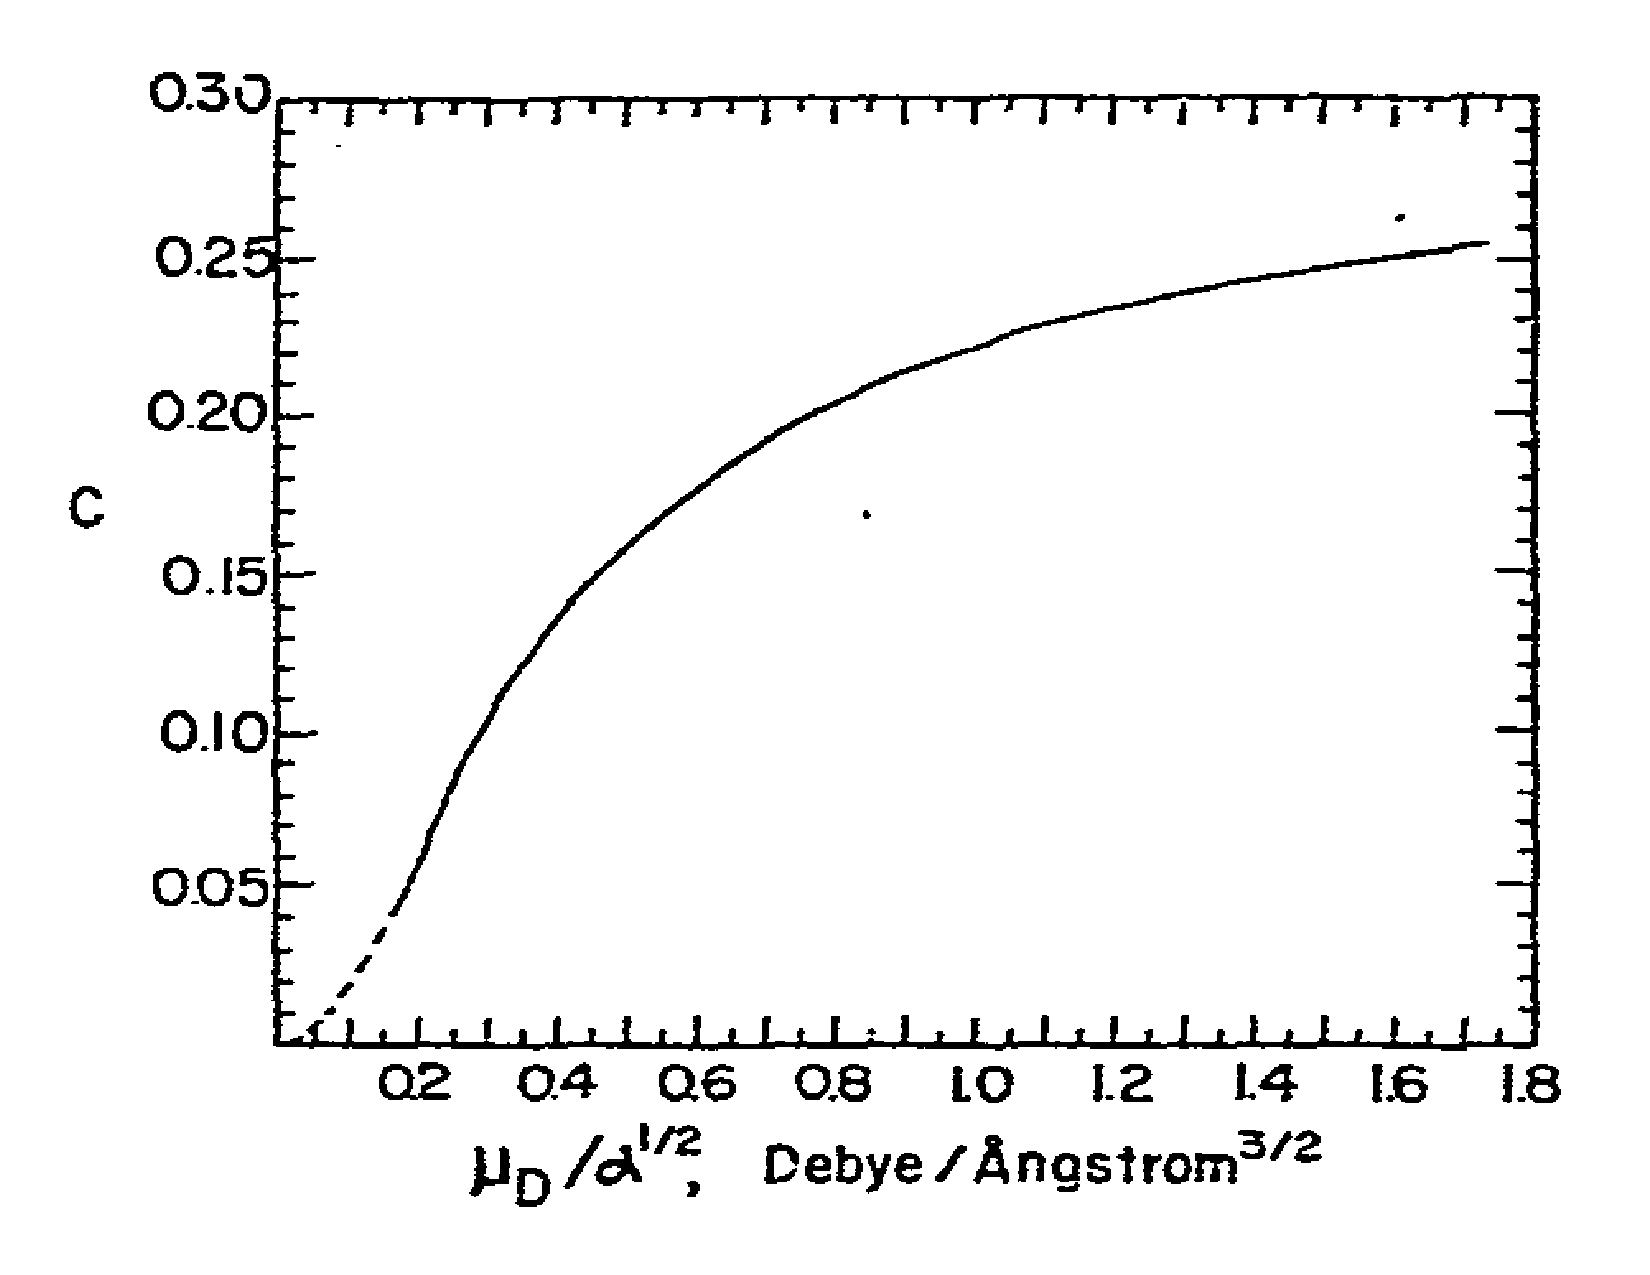
\includegraphics[width=0.8\textwidth]{images/ADO_C.pdf}
	\caption{Dipole locking constant $C$ parameterized by the dipole moment $\mu_D$ and polarizability $\alpha$. Figure taken from "Ion-polar molecule collisions: the effect of ion size on ion-polar molecule rate constants; the parameterization of the average-dipole-orientation theory" by Su et al.\cite{Su1973a}}
\end{figure}
